\section{System Design Overview}

\subsection{Scope and design goals}
This thesis designs and demonstrates a hospital management system (HMS) using a microservices architecture, with a focus on enforcing access control through a role-centric hybrid RBAC/ABAC model (RBAC-A) as presented in \cite{KuhnCoyneWeil2010}. The goal is to show how fine-grained authorization can be applied in a realistic hospital setting without making the system difficult to maintain.
\vspace{0.5cm}


To keep implementation and evaluation manageable for a bachelor thesis, the prototype scope is intentionally limited to seven core services that represent the most common clinical and administrative workflows. These services include the User Service for staff profiles and role bindings, the Patient Service for patient information and medical records, the Appointment Service for scheduling, the Lab Service for lab orders and results, the Pharmacy Service for prescriptions and dispensing, the Billing Service for invoices and payments, and the Audit Service for access logs. Each service follows independent data ownership (database per service). Supporting services that can exist in a full HMS (such as notifications or reporting) are not included because they are not required to demonstrate and evaluate the hybrid authorization model.
\vspace{0.5cm}


Even with this limited scope, the system still covers the main situations where access control matters most: viewing patient records, booking appointments, issuing and dispensing prescriptions, and handling billing. These workflows also differ in resource types and sensitivity, which makes them suitable for demonstrating policies that depend on both roles and context. At the same time, keeping the scope small helps keep the policy set understandable and testable.

\subsection{Actors}
\label{subsec:actors}
The prototype is built around common hospital roles and their daily tasks. Doctors access patient records, document clinical information, order lab tests, and issue prescriptions. Nurses support patient care and update information based on assigned duties. Receptionists handle appointment booking and basic administrative updates, typically without access to detailed medical content. Lab technicians create or update test status and publish lab results, mostly within the Lab Service. Pharmacists verify prescriptions and dispense medicine, with operations centered around prescription state and inventory updates. Billing clerks create invoices and record payments, and administrators manage users, roles, and authorization policies. The system also includes a patient role, which is usually restricted to viewing only personal information such as one’s own appointments and payment status.
\vspace{0.5cm}


These actors reflect a typical RBAC structure used in hospitals, but many real decisions still depend on attributes such as department, assignment, and time conditions. This is the motivation for combining RBAC with ABAC constraints in a controlled way.

\subsection{System Overview diagram}
Figure~\ref{fig:systemoverview} summarizes the overall system design using a layered view. The architecture separates client access, edge enforcement, authorization decision-making, and business microservices.


\subsubsection{Layer A — Client/UI:} Users interact with the system through the portal or mobile app. Authentication is handled by an Identity Provider that issues access tokens (JWT).

\subsubsection{Layer B — Edge:} The API Gateway/BFF acts as the primary Policy Enforcement Point (PEP). It intercepts incoming requests, validates the token, and requests an authorization decision before routing the request to a target service.

\subsubsection{Layer C — Authorization:} A centralized Authorization Service acts as the Policy Decision Point (PDP). It evaluates access requests using role-centric Hybrid RBAC/ABAC rules. Policy definitions and constraints are managed in a policy store, and required attributes/context can be provided via an attribute provider.

\subsubsection{Layer D — Business Services:} Domain microservices implement HMS business functions such as Patient record, scheduling, lab results, billing, pharmacy, etc. Each service owns its data store.

A typical request follows these steps:
\begin{itemize}
    \item The user logs in and receives a JWT from the Identity Provider.
    \item The client sends an HTTPS request with the JWT to the API Gateway/BFF.
    \item The Gateway sends an authorization decision request to the Authorization Service.
    \item The Authorization Service returns a Permit or Deny decision.
    \item If permitted, the Gateway routes the request to the target microservice.
\end{itemize}

\begin{figure}[H]
    \centering
    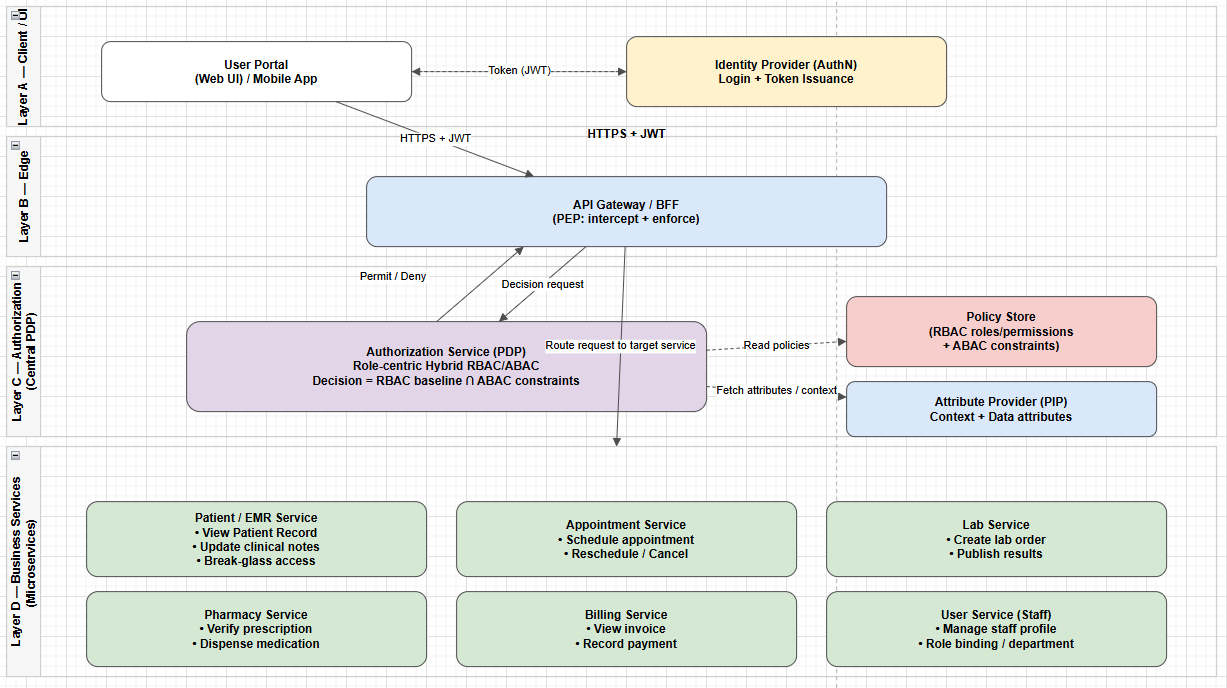
\includegraphics[width=1\linewidth]{images/systemoverview.png}
    \caption{System Overview Diagram}
    \label{fig:systemoverview}
\end{figure}
\section{System Architecture}
This section describes how the HMS prototype is structured and how requests move through the system. The design follows a microservices approach and uses a centralized authorization service (central PDP) to make access decisions consistently across services.

\subsection{Microservices decomposition}
The prototype is divided into seven business services with clear boundaries. The User Service stores staff profiles and organizational information that is relevant for authorization, such as department and job position. The Patient Service manages patient information and medical record data. The Appointment Service handles scheduling and appointment lifecycle. The Lab Service manages lab orders and results. The Pharmacy Service manages prescriptions and medication dispensing actions. The Billing Service handles invoices and payment records. Finally, the Audit Service records access decisions and request metadata to support traceability and compliance.
\vspace{0.5cm}


This decomposition is useful not only for modular development, but also for authorization clarity. Instead of treating the system as one large application, access can be controlled by resource type such as patient records, lab results, prescriptions, and invoices. This aligns well with hospital workflows and helps policies remain readable.


\subsection{Data ownership}
The application applies the database-per-service principle. Each microservice owns its database, and other services do not read it directly. Data sharing, when necessary, happens through APIs. This matters in a hospital setting because data is sensitive and should not be implicitly exposed through direct database access patterns.
\vspace{0.5cm}


At the same time, authorization decisions often require context from multiple sources. For example, a decision might depend on a staff member’s department (from the User Service) and a resource attribute such as the patient’s ward or record sensitivity (from the Patient Service). Instead of breaking data ownership by letting services query each other’s databases, this thesis uses an attribute provider pattern (PIP). The PIP retrieves only the minimal attributes needed for a decision by calling service APIs, which preserves isolation and reduces unintended data exposure.


\subsection{System Architecture Diagram}
\label{sec:sysarchitecture}
Figure~\ref{fig:archdiagram} illustrates the full architecture used in this thesis. The key idea is that enforcement happens at the edge, while decisions are evaluated centrally. This also defines a clear trust boundary: the client is not trusted to enforce access rules, so all requests must pass through the gateway.
\vspace{0.5cm}


The API Gateway/BFF is the main entry point for client requests and serves as the PEP. It validates JWT tokens, extracts basic identity claims, constructs an authorization decision request, calls the PDP, and forwards the request only when the result is Permit. Authentication is handled by an OIDC/OAuth2 Identity Provider, which manages users and roles and issues JWT tokens.
\vspace{0.5cm}


The Authorization Service is the PDP. It evaluates the role-centric hybrid model used in this thesis: RBAC provides the baseline role-to-permission mapping, and ABAC introduces constraints based on context and resource attributes. Policies are managed separately through a Policy Service (PAP) and stored in a dedicated policy database. The policy store acts as the source of truth, while OPA holds a deployed copy used for evaluation. When additional attributes are required, the PDP calls the PIP to fetch them from relevant domain services. Finally, the system records decision logs in the Audit Service to support traceability.

\subsubsection{API Gateway / BFF (PEP)}
The gateway is the entry point for client requests. It acts as the main enforcement point (PEP). Its job is:
\begin{itemize}
    \item receive HTTPS requests from clients,
    \item validate the access token (JWT),
    \item build an authorization request (who, what action, what resource, and basic context),
    \item ask the Authorization Service for a decision,
    \item only route the request to the target service if the decision is Permit.
\end{itemize}

\subsubsection{Identity Provider (Authentication)}
Authentication is handled by an identity provider (OIDC/OAuth2). Users log in and receive a JWT. The gateway uses this token to identify the user and extract basic claims.
\subsubsection{Authorization Service (PDP)}
This service is the decision point (PDP). It evaluates the hybrid model used in this thesis:
\begin{itemize}
    \item RBAC provides the baseline (role → permissions),
    \item ABAC adds constraints (context and data attributes).
\end{itemize}

The PDP returns \textbf{Permit/Deny}, and it may include simple obligations (e.g., logging requirements). The detailed policy logic is described later in Section 3.4.

\subsubsection{Policy Service (PAP) and Policy Store}
Policies are managed separately from business services. A policy admin updates policies through the PAP. Policies are stored in a dedicated policy store managed by the Policy Service, and the deployed policy set is published to OPA for evaluation by the PDP. This separates policy management from the application logic and keeps changes controlled.

\subsubsection{Attribute Provider (PIP)}
Some access decisions need extra data that is not in the JWT. For example: staff department, patient care-team relationship, and appointment assignment. The PIP fetches these attributes from the relevant services (User/Patient/Appointment). The PDP uses these attributes to evaluate ABAC constraints.
\subsubsection{Audit Service}
The system writes decision logs to an audit log store. This supports traceability, which is important in hospital systems. In this implementation, the audit flow is kept simple: it records the authorization decision and a small set of request metadata.
\begin{figure}[H]
    \centering
    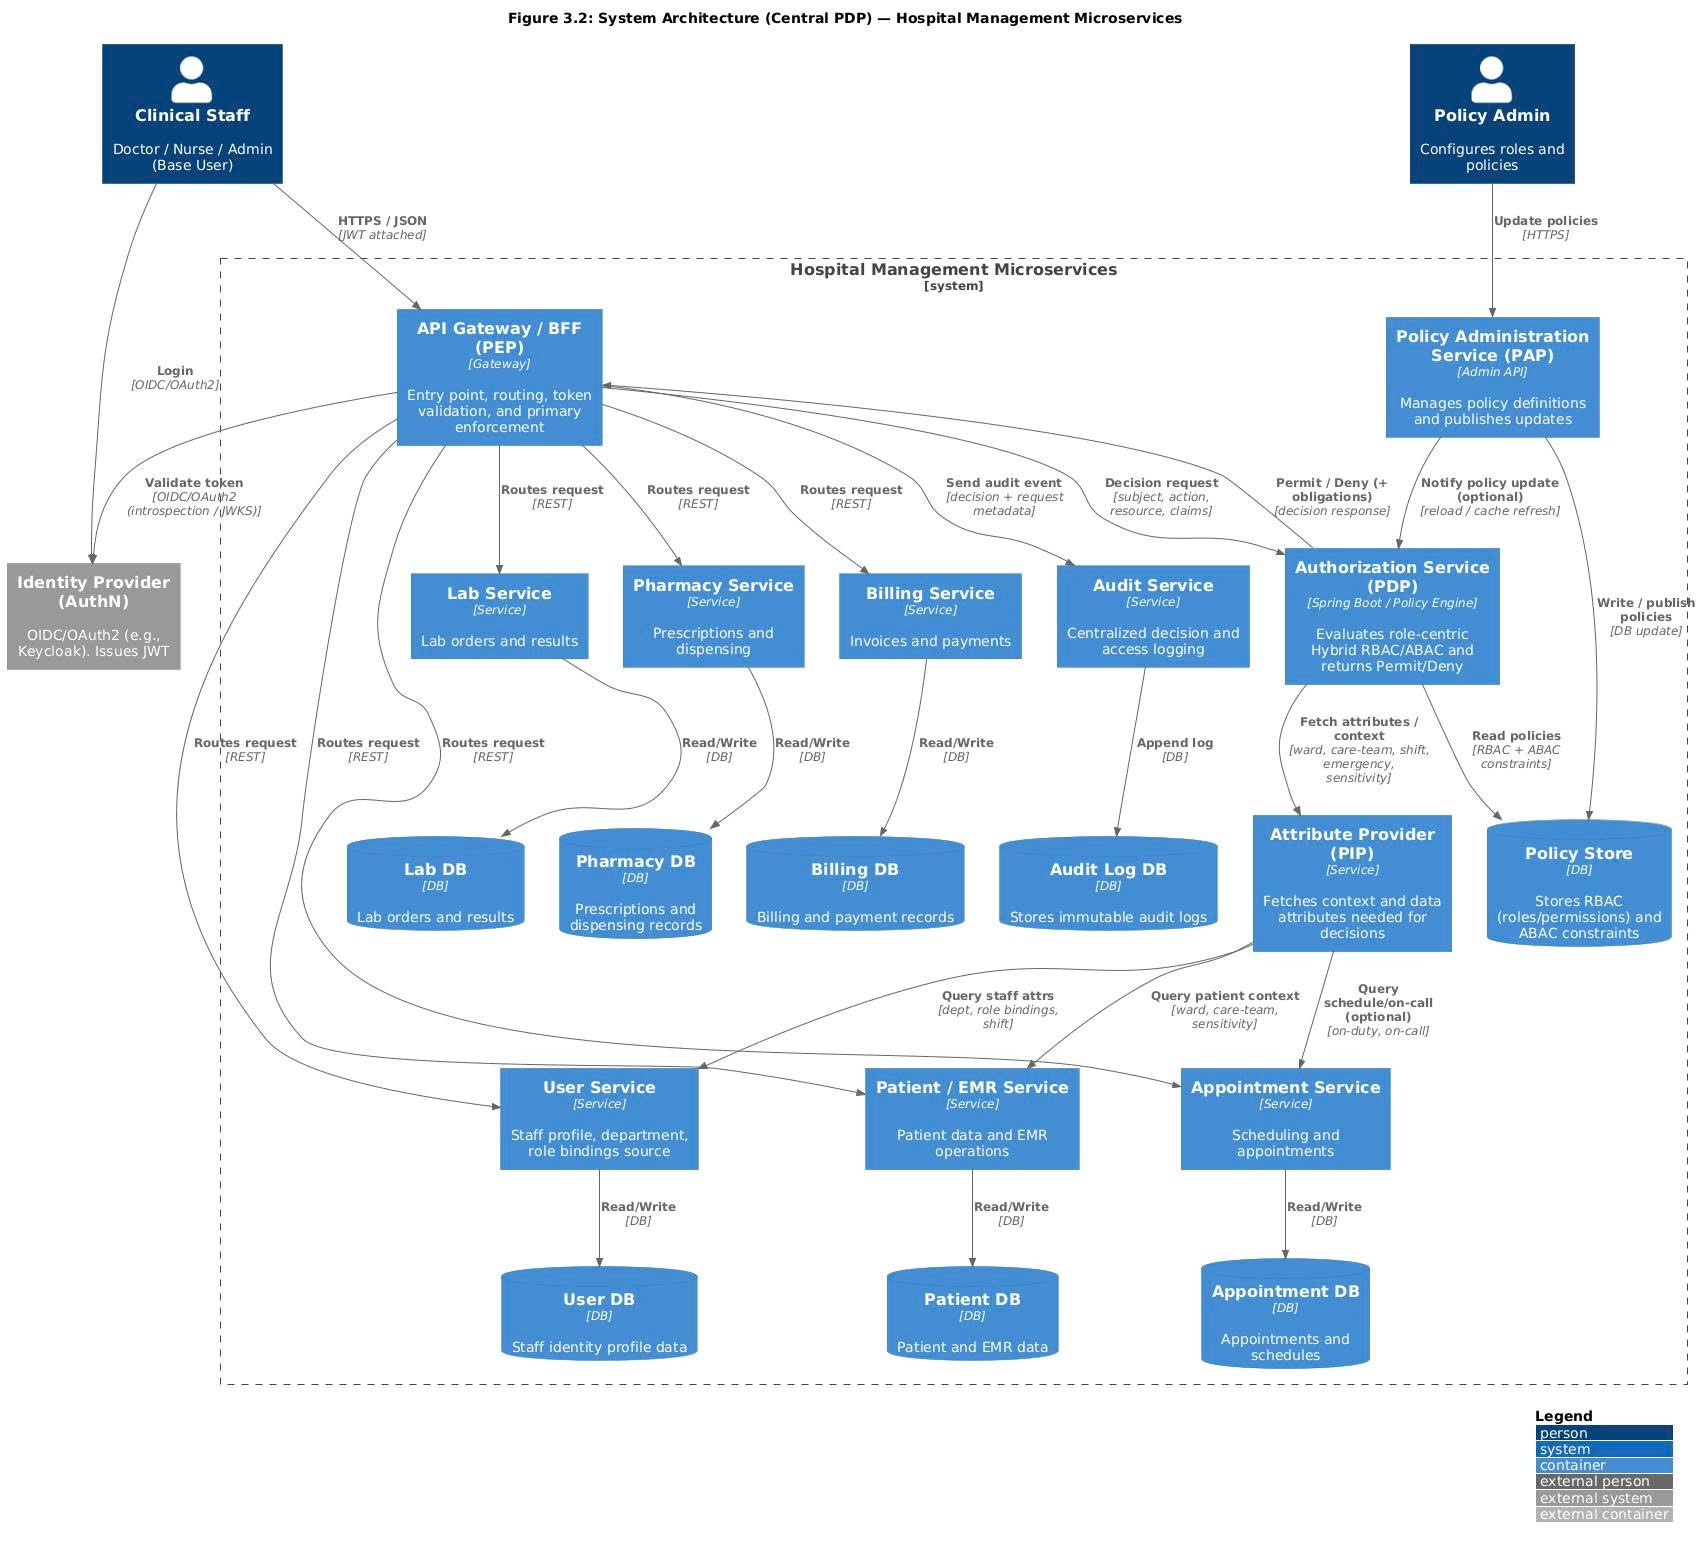
\includegraphics[width=1\linewidth]{images/architecturediagram.png}
    \caption{Architecture Diagram - Hospital Management Microservices}
    \label{fig:archdiagram}
\end{figure}
Figure~\ref{fig:archdiagram} also shows the trust boundary in the system. The client is not trusted to enforce access rules, so all requests must go through the gateway. Business services focus on domain logic and do not decide authorization on their own in this prototype. This keeps the behavior consistent: the same role and context should lead to the same Permit/Deny decision no matter which service is called.
\subsection{Authorization flow}
Figure~\ref{fig:seqdiagram} presents the request flow for a common HMS scenario: a doctor views a patient record. In this flow, the user has already logged in through the Identity Provider, so the client sends an HTTPS request with a valid JWT in the \texttt{Authorization: Bearer <JWT>} header. The gateway first validates the token and extracts basic claims such as user id and role. If the token is missing, expired, or invalid, the gateway stops the request early and returns \texttt{401 Unauthorized}.


\begin{figure}[H]
    \centering
    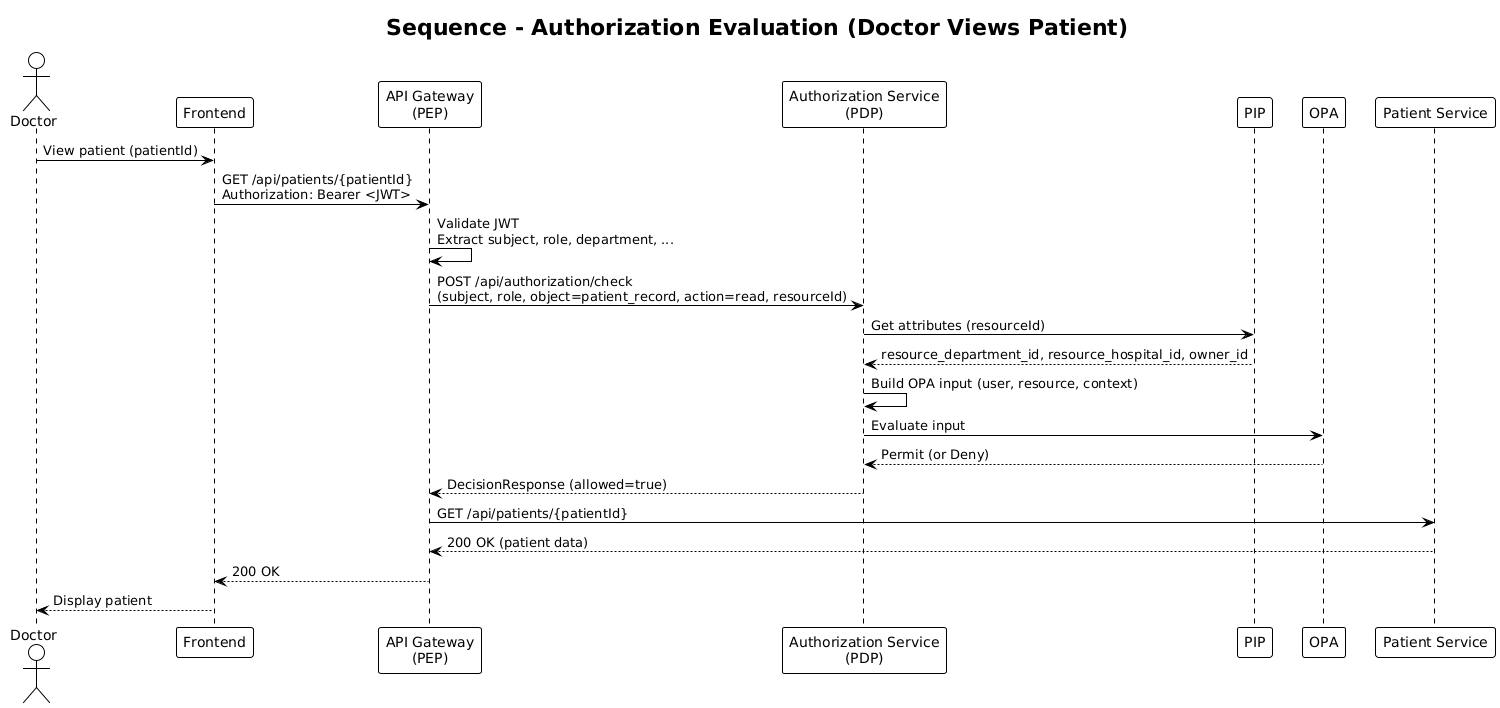
\includegraphics[width=1\linewidth]{images/sequencediagram.png}
    \caption{Sequence Diagram - Doctor View Patient}
    \label{fig:seqdiagram}
\end{figure}
When authentication succeeds, the gateway builds a decision request and sends it to the Authorization Service. The decision request captures the core information needed for authorization, including the subject, the requested action (such as \texttt{read} or \texttt{update}), the resource type and identifier (for example, \texttt{patient\_record} and \texttt{patientId}), and basic request context.
\vspace{0.5cm}


Next, the PDP requests additional attributes through the PIP when necessary. This is important because many hospital decisions cannot rely on JWT claims alone. For example, determining whether a doctor can access a specific patient record may require department matching, assignment information, or resource sensitivity flags. In this design, the PIP returns only the attributes required to evaluate constraints, not full domain payloads such as the complete medical record. This keeps authorization efficient and reduces the risk of exposing sensitive data during decision-making.
\vspace{0.5cm}


After collecting the needed attributes, the PDP builds the final policy input and evaluates it using the policy engine (OPA). OPA returns a Permit or Deny decision, optionally with small metadata for logging and debugging. The gateway then enforces the result: it forwards the original request only when access is permitted, and otherwise returns a forbidden response without calling the business service. The same pattern applies to other protected actions such as dispensing medication or creating an invoice. What changes across workflows is mainly which attributes are required for ABAC constraints.

\section{Key Workflows and Use Cases}
This section highlights representative workflows that are used later for implementation and evaluation. The intention is to show where RBAC is sufficient, where it becomes too rigid, and how the hybrid RBAC-A design helps by adding constraints in a controlled way. Diagrams provide a quick view of the flow, while short descriptions clarify how authorization is applied before state-changing operations reach domain services.


\subsection{Authorization and policy management}
\label{subsec:workflow_auth_policy}
Figure~\ref{fig:activityauthorization} illustrates how a protected request is evaluated by the system. The design separates enforcement from decision-making. The gateway enforces the outcome by allowing or blocking traffic, while the PDP evaluates policy logic and constraints. This separation keeps business services unchanged and avoids duplicating authorization checks inside every microservice.

\begin{figure}[H]
    \centering
    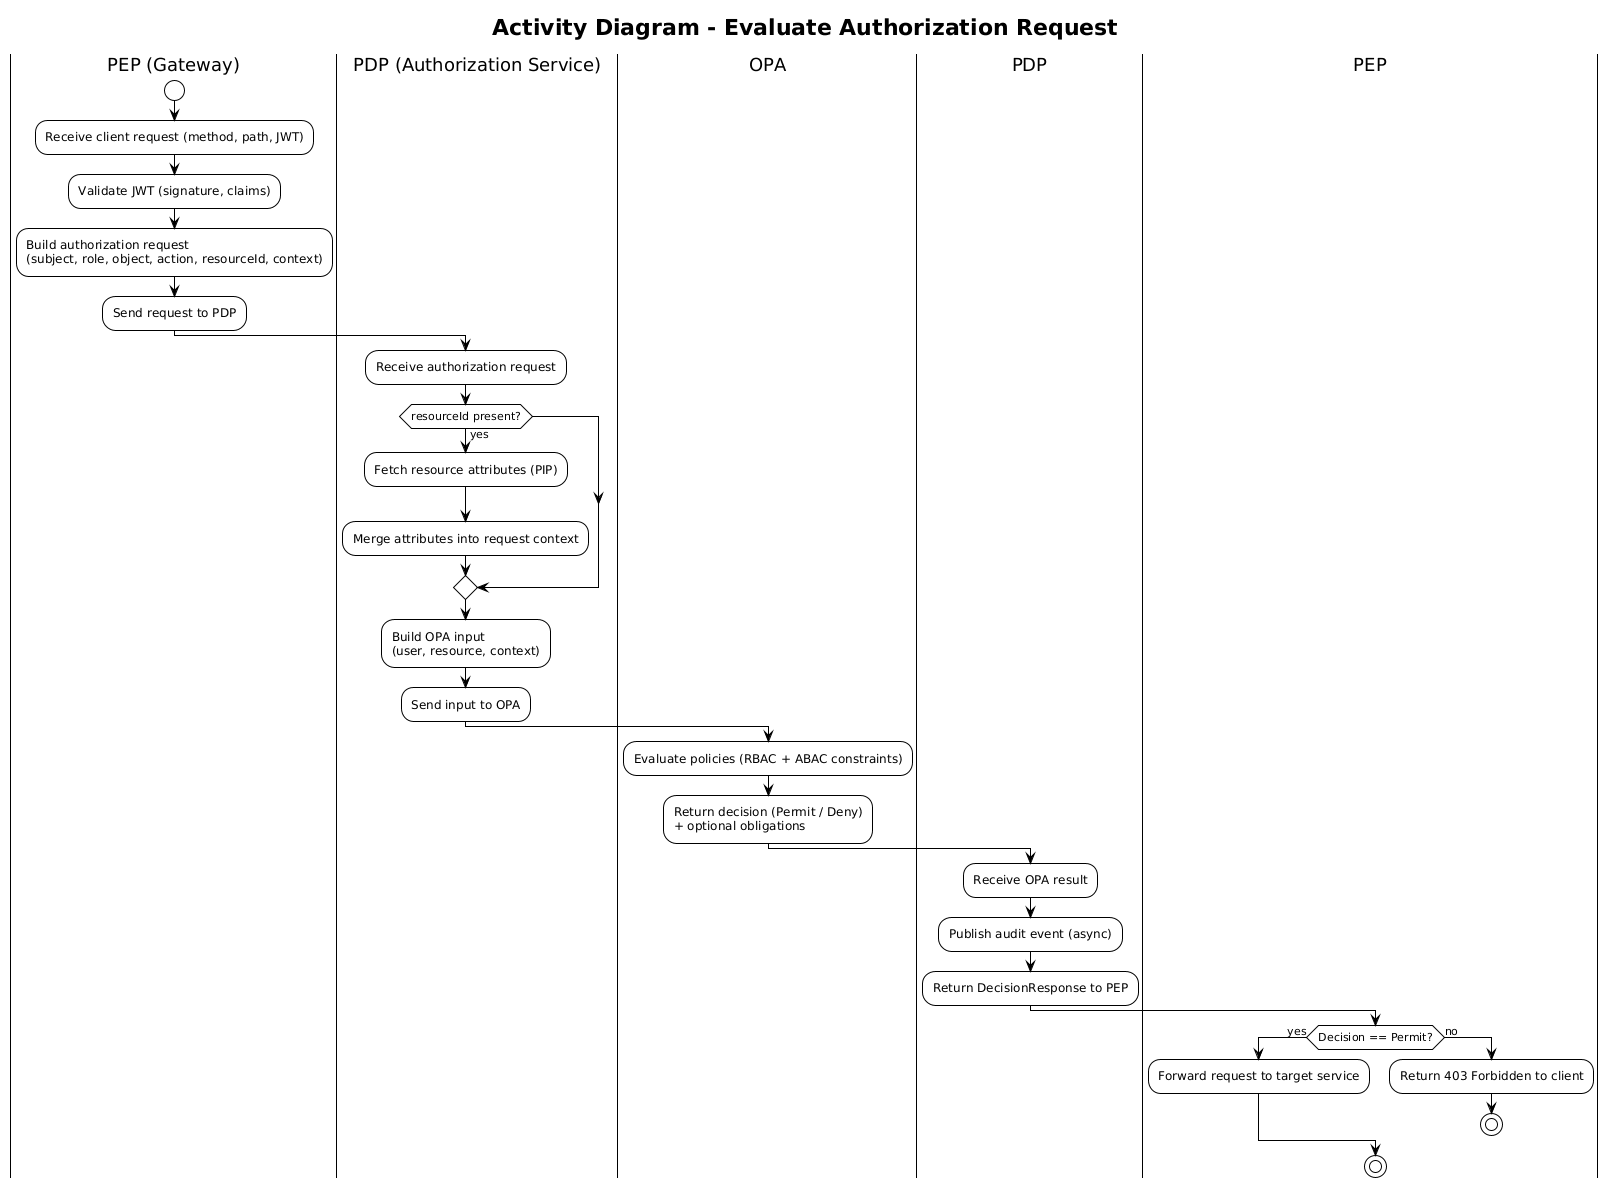
\includegraphics[width=1\linewidth]{images/activityauthorization.png}
    \caption{Activity Diagram - Evaluate Authorization Request}
    \label{fig:activityauthorization}
\end{figure}
In practice, the gateway translates an HTTP request into a decision request that contains the subject, action, resource, and basic context. The PDP enriches the request with missing attributes through the PIP when needed and evaluates constraints using OPA. If the final result is Deny, the request is stopped at the gateway and never reaches the target service. This is important because it reduces the chance of partial information leakage, such as revealing service behavior through timing differences or detailed error responses.
\subsection{Appointment Management}
\subsubsection{Use case diagram}
Booking an appointment is a workflow where RBAC alone is often not enough. Multiple roles may create an appointment, such as patients and receptionists, but the action should still be constrained by hospital scope, department, and other context. Figure~\ref{fig:usecaseappointment} shows the use case view for appointment booking. In this thesis, the action is modeled as \texttt{appointment:create} and the resource type is \texttt{appointment}. The authorization check is performed before the Appointment Service proceeds with slot availability checks and appointment creation.

\begin{figure}[H]
    \centering
    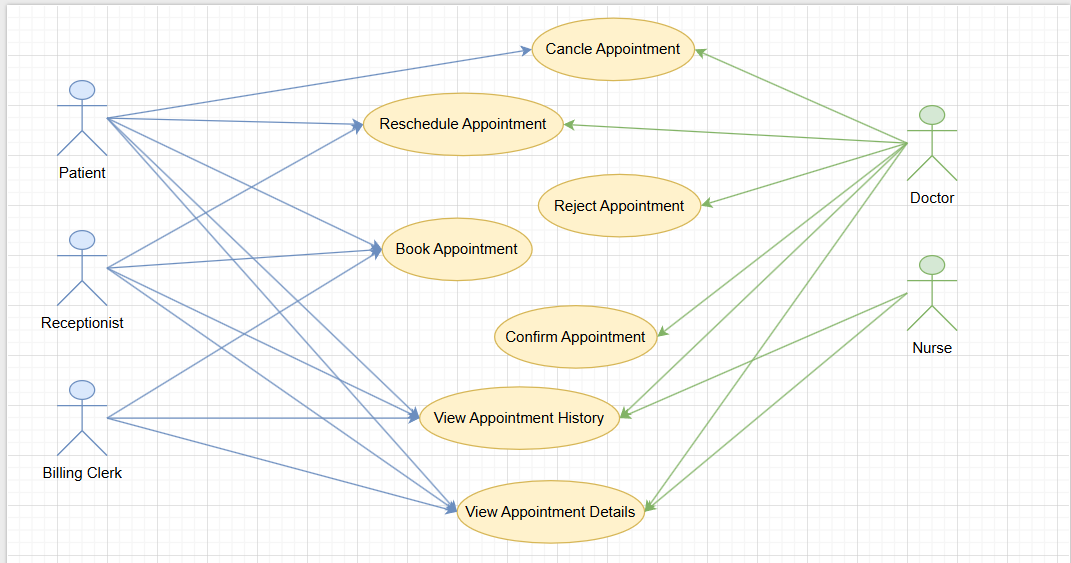
\includegraphics[width=1\linewidth]{images/use-case-appointment.png}
    \caption{Use Case Diagram - Booking Appointment}
    \label{fig:usecaseappointment}
\end{figure}


\subsubsection{Use case table}
\begin{table}[H]
\centering
\label{tab:uc-appointment}
\begin{tabular}{|l|p{9cm}|}
\hline
\textbf{Name} & \textbf{Description} \\
\hline
Actor & Patient, Receptionist, Billing Clerk, Doctor, Nurse \\
\hline
Main function & Book Appointment \\
\hline
Brief description & The Receptionist (or Patient) selects a patient and a preferred time slot, then submits a booking request. The system checks the user's authorization (role and context) and the availability of the slot. If permitted and the slot is available, a new appointment is created with status PENDING\_CONFIRMATION. The Doctor may later Confirm or Reject the appointment. \\
\hline
Context information & User is logged in; appointment management module is available. Patient and doctor/department are known. \\
\hline
\end{tabular}

\end{table}




\begin{table}[H]
\centering
\begin{tabular}{|l|p{9cm}|}
\hline
\textbf{Name} & \textbf{Description} \\
\hline
Triggers & User must be authenticated (JWT). User must have permission to create appointments (e.g. Receptionist, Billing Clerk, or Patient role). At least one time slot must be selectable. \\
\hline
Flow of events summary & 
1. Receptionist or Patient opens the appointment booking page. \\
& 2. User selects patient (if Receptionist/Billing Clerk) and preferred date/time slot. \\
& 3. User submits the booking request. \\
& 4. System (PEP) validates JWT and sends an authorization request to the PDP. \\
& 5. PDP evaluates RBAC and ABAC; if Deny, system returns \texttt{403 Forbidden}. \\
& 6. System checks slot availability in the Appointment Service. \\
& 7. If the slot is available, system creates the appointment and returns confirmation. \\
& 8. Doctor may later confirm or reject the appointment. \\
\hline
\end{tabular}
\caption{Use case table: Book Appointment (Appointment Management)}
\label{tab:uc-appointment}
\end{table}
\vspace{1em}







\subsubsection{Activity Diagram}
\begin{figure}[H]
    \centering
    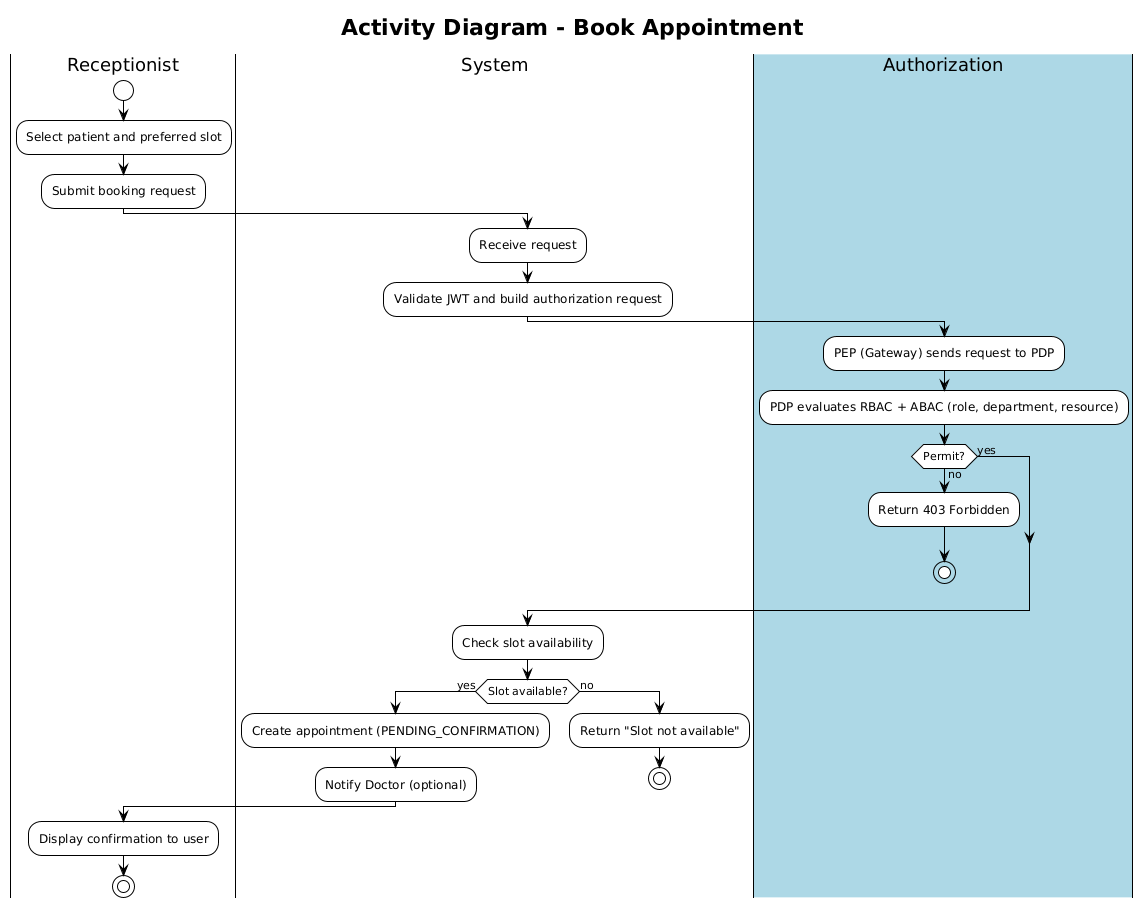
\includegraphics[width=0.75\linewidth]{images/activity-appointment.png}
    \caption{Activity Diagram - Booking Appointment - Receptionist}
    \label{fig:activityappointment}
\end{figure}



\subsubsection{Sequence Diagram}
\begin{figure}[H]
    \centering
    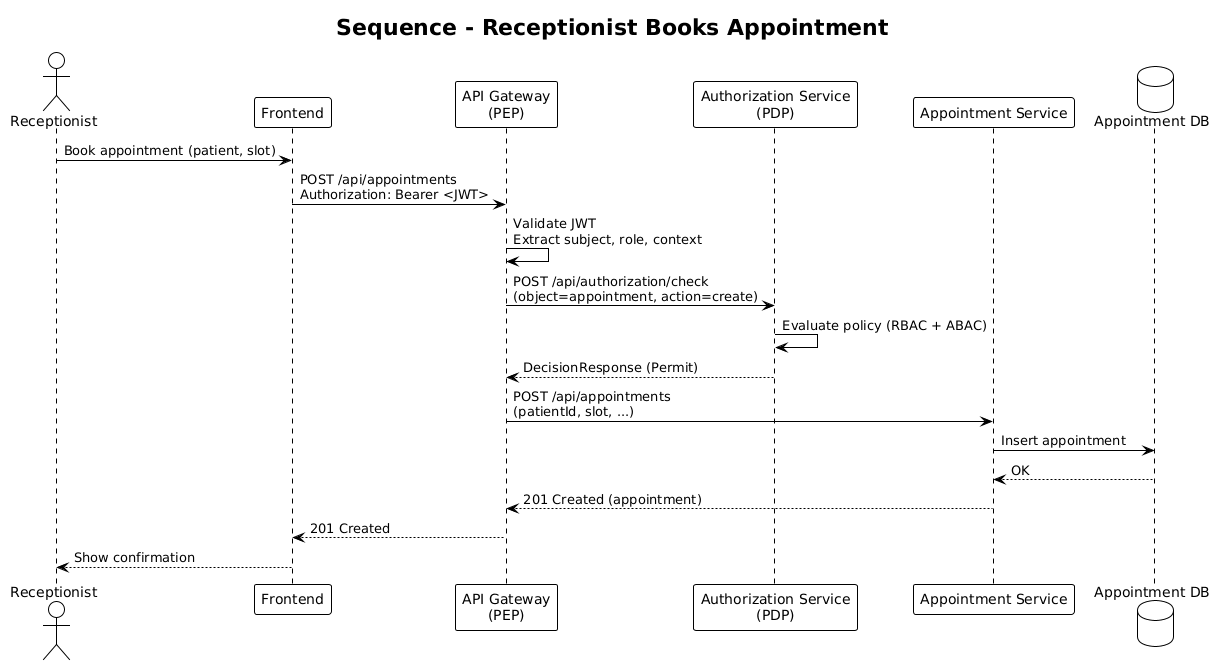
\includegraphics[width=1\linewidth]{images/sequence-appointment.png}
    \caption{Sequence Diagram - Booking Appointment - Receptionist}
    \label{fig:seqappointment}
\end{figure}
In this workflow, the receptionist selects a patient and a preferred time slot, then submits a booking request through the UI. The request goes to the gateway, which validates the JWT and asks the PDP for a decision. If the decision is Deny, the system stops early. If it is Permit, the Appointment Service continues by checking whether the slot is available and then creates a new appointment with status \texttt{PENDING\_CONFIRMATION}. A doctor can later confirm or reject the appointment, which introduces a second set of actions with different authorization requirements.


\subsection{Prescription \& Pharmacy }
Dispensing medication is sensitive because it changes prescription state and inventory records. RBAC provides the baseline permission (for example, a pharmacist role is allowed to dispense), but ABAC constraints can narrow access based on hospital scope, working hours, or prescription type. Figure~\ref{fig:usecasepharmacy} illustrates the prescription and pharmacy use case view. In this workflow, the authorization request is modeled as resource type \texttt{prescription} and action \texttt{dispense}. The Pharmacy Service performs the state change only after the gateway receives a Permit decision.


\subsubsection{Use case Diagram}

\begin{figure}[H]
    \centering
    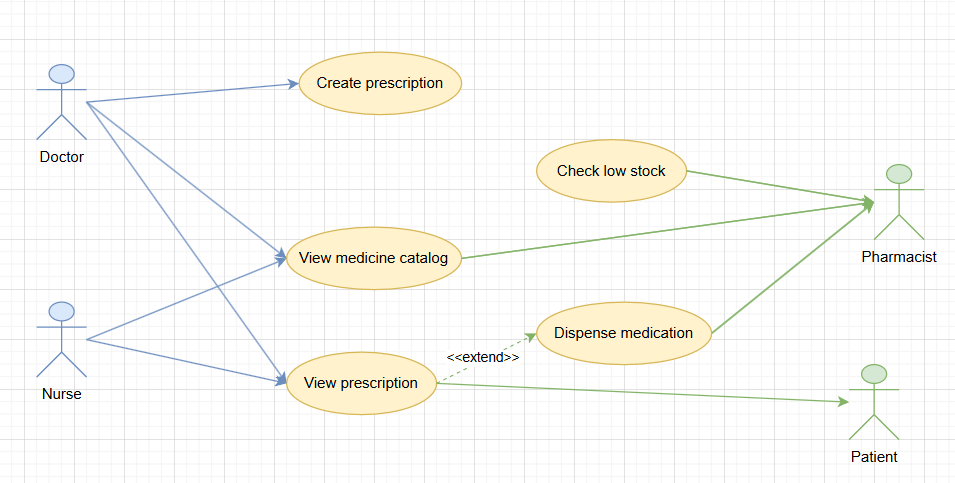
\includegraphics[width=1\linewidth]{images/use-case-diagram-pharmacy.png}
    \caption{Use case diagram - Prescription \& Pharmacy}
    \label{fig:usecasepharmacy}
\end{figure}

\subsubsection{Use case table}


\begin{table}[H]
\centering
\begin{tabular}{|l|p{9cm}|}
\hline
\textbf{Name} & \textbf{Description} \\
\hline
Actor & Pharmacist \\
\hline
Main function & Dispense Medication \\
\hline
Brief description & The Pharmacist selects a prescription that is in APPROVED status, verifies patient allergies and medicine stock, then confirms the dispense action. The system updates the prescription status to DISPENSED, records the dispenser and timestamp, deducts the quantity from inventory, and creates an inventory transaction (OUT). \\
\hline
Context information & Prescription exists and has been approved by a Doctor. Medicine is available in the pharmacy inventory. \\
\hline
Triggers & User must be authenticated and have the Pharmacist (or Admin) role. The prescription must be in APPROVED status. The requested medicine and quantity must be in stock. \\
\hline
\end{tabular}

\label{tab:uc-prescription-1}

\end{table}



\begin{table}[H]
\centering
\begin{tabular}{|l|p{9cm}|}
\hline
\textbf{Name} & \textbf{Description} \\
\hline
Flow of events summary & 
1. Pharmacist opens the list of approved prescriptions. \\
& 2. Pharmacist selects a prescription to dispense. \\
& 3. System validates authorization (PEP $\rightarrow$ PDP); if Deny, access is refused. \\
& 4. Pharmacist reviews prescription details and (if shown) patient allergies. \\
& 5. Pharmacist verifies that the medicine and quantity are available in stock. \\
& 6. Pharmacist confirms the dispense action. \\
& 7. System updates prescription status to DISPENSED and records dispensed\_by, dispensed\_at. \\
& 8. System deducts quantity from inventory and creates an OUT transaction. \\
& 9. System returns success to the Pharmacist. \\
\hline
\end{tabular}
\caption{Use case table: Dispense Medication (Prescription \& Pharmacy)}
\label{tab:uc-prescription}

\end{table}
\vspace{1em}


\subsubsection{Activity Diagram}

\begin{figure}[H]
    \centering
    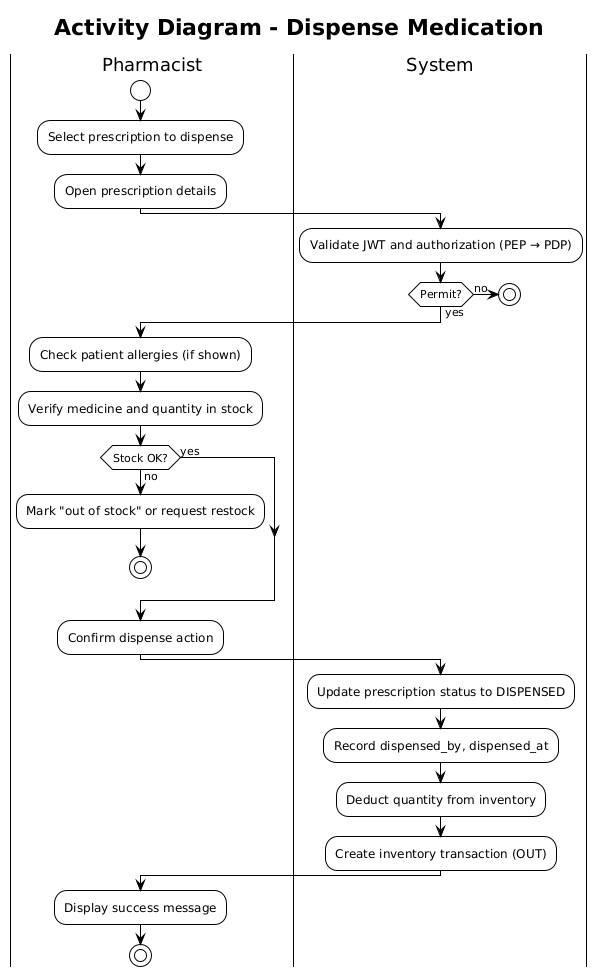
\includegraphics[width=0.5\linewidth]{images/actitvitypharmacy.png}
    \caption{Activity Diagram - Dispense Medication}
    \label{fig:activitypharmacy}
\end{figure}
A typical dispensing flow starts when the pharmacist opens the list of approved prescriptions and selects one to dispense. The system evaluates authorization before performing any updates. If permitted, the pharmacist verifies prescription details and stock availability, then confirms the dispensing action. The system updates the prescription status to \texttt{DISPENSED}, records the dispenser and timestamp, deducts the quantity from inventory, and creates an inventory transaction record. By placing authorization in front of these state changes, the system reduces the risk of unintended updates and keeps enforcement consistent.

\section{Hybrid Access Control Design}

\subsection{Model Selection}
In hospital systems, access control must balance two needs. First, patient data is highly sensitive, so access must be restricted and auditable. Second, clinical work is time-critical, so the model must remain practical to manage and fast enough for daily use. Traditional RBAC is widely used because it is easy to review and administer once roles and permissions are defined. However, RBAC alone becomes rigid when access depends on context such as time, shift, assignment, or department. When RBAC tries to cover many contexts by introducing more roles, it can lead to role explosion (too many roles to maintain). \cite{KuhnCoyneWeil2010, Ferraiolo2007RBAC2E}
\vspace{0.5cm}


ABAC is more flexible because it can express rules directly using attributes, but it can be difficult to manage at scale. \cite{KuhnCoyneWeil2010} points out that ABAC’s flexibility comes with a cost: many attribute combinations may need to be considered, and it can be hard to analyze “who has what permissions” for a given employee position.
\vspace{0.5cm}


To combine the strengths of both models, this thesis adopts RBAC-A (role-centric), as described by \cite{KuhnCoyneWeil2010}. In RBAC-A, roles still define the maximum permission set, while attributes are added as constraints. In the role-centric variant, attribute-based rules can only reduce the permissions available to a user; they do not expand access beyond what the role already allows.
\vspace{0.5cm}


\cite{KuhnCoyneWeil2010} summarize several integration options and describe the role-centric approach as the mapping:


\textbf{User → Role → Attributes → Permission decision }

Under this approach, the final permission set is computed as an intersection:

\begin{itemize}
    \item let \emph{P} be the set of permissions granted by active roles (RBAC baseline),
    \item let \emph{R} be the set of permissions allowed after applying attribute constraints (ABAC rules),
then the effective permissions are $P \cap $R
\end{itemize}
This is the key reason this thesis selects role-centric RBAC-A: it keeps RBAC’s administrative clarity (roles remain the main unit of review), while adding enough flexibility to handle common hospital contexts (time, department, owner, and so on). 

\subsection{Policy Evaluation Workflow (PEP–PDP–PIP)}
Figure~\ref{fig:peppippdp} summarizes how the prototype evaluates authorization decisions. The gateway acts as the PEP and intercepts each request. It validates the JWT and extracts basic claims such as user id and roles. The gateway then sends a decision request to the Authorization Service, which acts as the PDP. When the decision requires context beyond what the token contains, the PDP queries the PIP for additional attributes, for example to check whether a doctor is assigned to a patient. After collecting the required attributes, the PDP evaluates the policy using OPA and returns a Permit/Deny result. The gateway enforces the result by forwarding the request only when access is permitted. 


\begin{figure}[H]
    \centering
    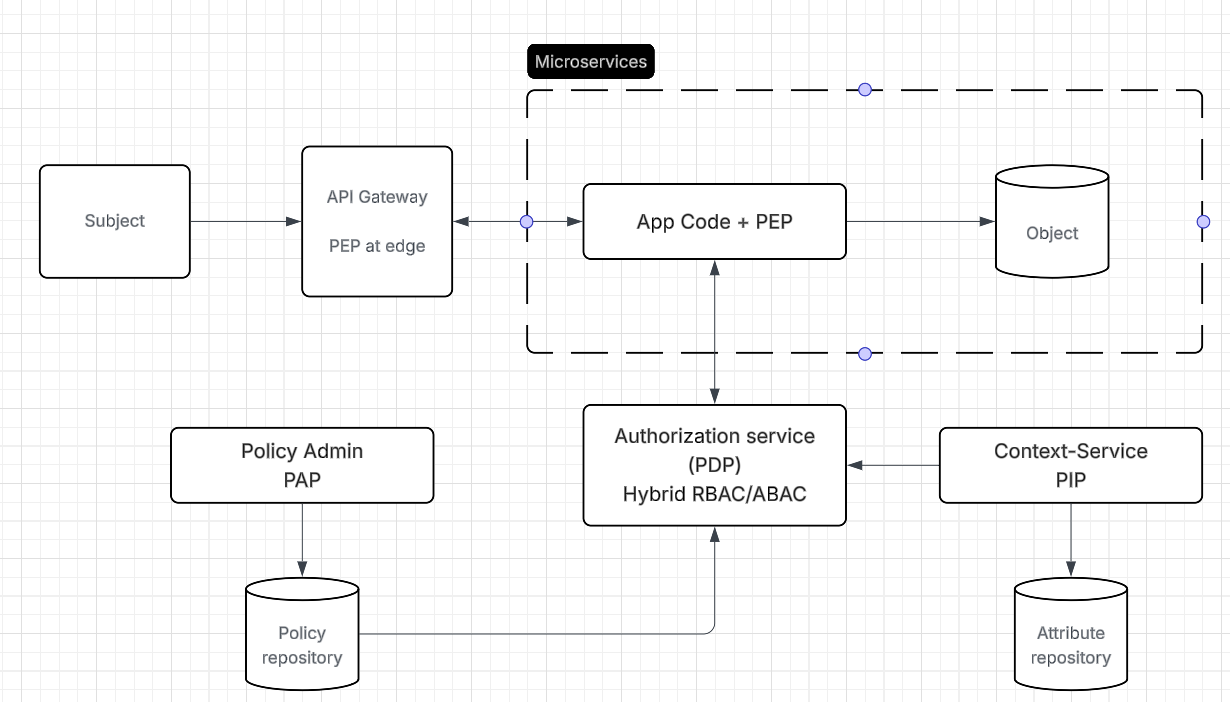
\includegraphics[width=0.75\linewidth]{images/peppippdp.png}
    \caption{System architecture for hybrid RBAC/ABAC authorization}
    \label{fig:peppippdp}
\end{figure}

This workflow protects business services consistently while keeping policy logic centralized and easier to maintain.

\subsection{Policy structure \& combining strategy}
Policies in this thesis follow the role-centric RBAC-A idea: roles define the baseline actions that are generally allowed on each resource type, and attributes narrow access through constraints such as time windows, department matching, or other context. The decision logic therefore happens in two stages. First, the system checks whether the user’s role allows the requested operation on the resource type. If the RBAC baseline fails, the request is denied immediately. If the RBAC baseline passes, the system evaluates ABAC constraints using the attributes collected through the PIP.
\vspace{0.5cm}


When more than one rule or policy can match a request, the system needs a clear and predictable combining behavior. In this thesis, matching rules are first evaluated within their parent policy according to that policy’s combining algorithm (e.g.\ \texttt{deny-overrides}, \texttt{allow-overrides}, or \texttt{first-applicable} based on priority). After that, the system resolves the final decision across matched rules using deterministic priority: deny rules take precedence; otherwise, the highest-priority allow rule wins. This separation keeps evaluation predictable while still allowing policies to be written in a practical format for administration and testing.

\subsection{Attribute model (Subject–Resource–Action–Context)}
\label{sec:hybrid-access-control-design}
The hybrid model in this thesis organizes attributes into four groups. Subject attributes represent who is making the request, such as user id, role, department, and staff-related fields. Resource attributes describe what data is being accessed, such as resource type, resource id, owner id, department id, or status fields that belong to domain objects. The action describes what operation is being requested, such as \texttt{read}, \texttt{create}, or \texttt{update}. Context attributes represent runtime conditions such as time or shift, device information, and IP or location indicators.
\vspace{0.5cm}

\paragraph{Reasons for the chosen attributes:}
The hybrid model in this thesis organizes attributes into four groups. Subject attributes represent who is making the request, such as user id, role, department, and staff-related fields. Resource attributes describe what data is being accessed, such as resource type, resource id, owner id, department id, or status fields that belong to domain objects. The action describes what operation is being requested, such as \texttt{read}, \texttt{create}, or \texttt{update}. Context attributes represent runtime conditions such as time or shift, device information, and IP or location indicators.
\vspace{0.5cm}


The PIP is responsible for collecting only the minimum attributes required to evaluate constraints. It should not return full business payloads, especially for sensitive resources. This design keeps authorization focused on decision-making while limiting unnecessary exposure of medical data.





\subsection{Policy conflict detection}
\label{sec:policy-conflict-detection}
When many policies are defined, some rules can apply to the same request but return different decisions. For example, one rule may allow access for a given role and resource in a time window, and another may deny the same. That situation is called a \emph{policy conflict}. If conflicts are not detected, the system can behave in an unpredictable way: the same kind of request might be allowed or denied depending on the order of evaluation or the combining algorithm. In practice, security problems often come from wrong or inconsistent policy configuration rather than from cryptographic failures~\cite{Zheng2019ABAC}. So we need a way to find conflicts before or after policy changes. The idea is simple: (1) find pairs of rules whose conditions can overlap (i.e.\ there exists at least one request that matches both), and (2) among those, report pairs where one rule permits and the other denies. The result is a list of conflicting rule pairs that an administrator can review and fix.
\vspace{0.5cm}

Because the number of rules can be large, comparing every pair of rules is expensive. Two approaches from the literature help. The first is \emph{rule reduction}: drop or ignore rules that cannot take part in any conflict (e.g.\ rules without actions or without subject/object attributes), and only run conflict checks on the remaining set~\cite{Shu2009Conflicts}. The second is to encode each rule (or its attribute conditions) into a compact form and use fast operations to test overlap.\cite{Zheng2019ABAC} represents attribute conditions as binary sequences and use bitwise AND to detect overlap between two rules, which speeds up conflict detection when the policy set and the number of attributes grow.
\vspace{0.5cm}


In this thesis, conflict detection is implemented in the policy service. When an administrator adds or updates policies, the system can run a conflict check (on demand or after save). The implementation uses rule reduction: only rules that have actions and at least subject or object attributes are considered. Rules are grouped by resource type and action so that we only compare rules that share at least one action and can apply to the same resource type. For each candidate pair (one Allow, one Deny), the service checks whether their subject and object attribute sets overlap; if time conditions are present, it also checks whether their time intervals overlap, using a binary-search style check on disjoint time intervals. In addition, \emph{redundancy} is detected: two rules with the same effect (both Allow or both Deny) that have fully overlapping conditions. Redundancy does not change the decision but makes the policy set harder to maintain; reporting it helps the administrator simplify policies~\cite{Zheng2019ABAC}. The output of the detector is a list of conflicting pairs (and optionally a ``witness'' request that matches both rules), so the admin can adjust or merge rules and redeploy.

\subsection{Policy governance and misuse prevention}
\label{sec:policy-governance}

The role-centric hybrid model in this thesis helps address the practical problem of role explosion. However, a hybrid system also introduces a second class of risks: \textbf{policy governance risks}. If policy changes are not controlled, hybrid rules can become inconsistent over time, and privileged users can abuse their power by creating overly broad Allow rules or by weakening constraints and conditions during policy updates. In a hospital setting, this is serious because the most harmful failures are \emph{false-permit} decisions (access granted when it should have been denied).
\vspace{0.5cm}

This thesis therefore treats governance as part of the access control design. The goal is to keep authorization behavior predictable, make policy changes traceable, and reduce the chance that a single administrator action silently weakens security. To address the concern that hybrid (RBAC \& ABAC) implementation must be \emph{effectively controlled}---and not only mentioned---we define what constitutes misuse and how the following controls prevent it.
\vspace{0.5cm}

\paragraph{Misuse and abuse in this context.}
We define \textbf{policy misuse} or \textbf{abuse of power} in the hybrid system as: (i) introducing into the enabled policy set a pair of rules that form an \emph{authorization conflict} (one Allow and one Deny for the same request conditions, as in Section~\ref{sec:policy-conflict-detection}), which makes access behavior unpredictable; or (ii) allowing policy write operations by subjects who are not authorized to administer policies, so that the system cannot attribute or limit who changes rules. The governance controls below are designed so that (i) is prevented by conflict checks on update, and (ii) is prevented by restricting policy writes to administrators.
\vspace{0.5cm}

\paragraph{Invariants and policy-update conditions.}
The design maintains two invariants. \textbf{Conflict-freedom:} at every point in time, the set of enabled policies does not contain any pair of rules that form an AUTH\_CONFLICT (overlapping conditions with opposite effects). \textbf{Write-restriction:} only subjects with the ADMIN role may perform create, update, or delete on policies. For a \emph{policy update} (create or update), the pre-condition is: the subject has role ADMIN; and, when conflict-on-save is enabled in strict mode, the proposed policy set (existing enabled plus the new or updated policy) must not contain any AUTH\_CONFLICT. The post-condition after a successful save is that the conflict-freedom invariant holds and the policy record has updated version, timestamps, and administrator identity (created\_by / updated\_by) for traceability.
\vspace{0.5cm}

\subsubsection*{Deterministic decision semantics (avoid ambiguous behavior)}
The first governance control is making the decision semantics explicit. In this thesis, evaluation is deterministic in two ways. First, the system follows the role-centric RBAC-A principle: ABAC constraints \emph{only narrow} access. If the RBAC baseline does not allow an action for the role, the request is denied immediately. Second, when multiple rules can match, the policy engine applies a defined combining strategy (e.g. \texttt{deny-overrides}, \texttt{allow-overrides}, or \texttt{first-applicable} within a policy), and then resolves the final result using a clear precedence: deny rules take priority; otherwise, the highest-priority allow rule applies. This reduces the risk of ``accidental permission'' caused by unclear rule ordering and supports predictable behavior so that misuse (e.g.\ unintended broadening of access) is easier to detect and audit.
\vspace{0.5cm}

\subsubsection*{Restricted policy administration (limit who can change rules)}
The second control is limiting who can create or update policies. In the prototype, policy write operations are restricted to administrators. This directly enforces the write-restriction invariant and prevents abuse by non-admin users (only ADMIN can change rules). This includes creating policies, updating policies, triggering OPA synchronization, and running conflict detection. Read-only access (listing and viewing policies) can be granted more widely for transparency, but write access is treated as a privileged action.
\vspace{0.5cm}

This separation matters because policy administration is a powerful capability. If too many users can edit policies, the system becomes hard to control and easy to misuse.
\vspace{0.5cm}

\subsubsection*{Change traceability and policy version history}
Hybrid systems evolve. New endpoints are added, services change, and hospital workflows change. For that reason, policy governance must support traceability. In this thesis, policies are stored with metadata that supports auditing and rollback: \texttt{enabled} state, \texttt{version}, timestamps, and the administrator identity (created/updated by). Metadata (e.g.\ \texttt{created\_at}, \texttt{updated\_at}, \texttt{created\_by\_keycloak\_id}, \texttt{updated\_by\_keycloak\_id}) creates a clear trail of \emph{who changed what and when}, which is necessary when investigating incidents or reviewing why access changed after a deployment. Full content snapshots for each version can be added in future work to support rollback; the current prototype relies on version and actor metadata for accountability.
\vspace{0.5cm}

\subsubsection*{Conflict checks on policy update (fail safe by default)}
The most direct way to control conflict risk is to detect it at the time of change. In this prototype, conflict detection is not only a reporting tool; it is also used as a guardrail. Before saving a new or updated policy, the policy service runs conflict detection on the proposed state (existing enabled rules plus the proposed change) when configured in \emph{strict} mode. If the change introduces an authorization conflict (Allow/Deny overlap on the same action and resource type under overlapping attribute conditions), the update is \textbf{rejected} and the service returns HTTP 409 with a conflict report; no change is persisted, so the conflict-freedom invariant is preserved. This prevents administrators from accidentally publishing policies that make access behavior unpredictable and directly addresses misuse (i).
\vspace{0.5cm}

This ``conflict-on-save'' approach is intentionally conservative. It prefers a safe failure (do not apply risky policy changes) over silently deploying a policy set with unclear behavior.
\vspace{0.5cm}

\subsubsection*{Audit evidence for sensitive access and privileged operations}
Finally, governance requires evidence. The authorization path records audit information for protected requests, including the final Permit/Deny decision and the context used for evaluation. For privileged events (for example policy updates, conflict scans, or access to audit logs), audit data is especially important because it supports accountability and later review. Policy create/update events can be sent to the audit service so that every change to the policy set is logged; this closes the loop from governance design to observable evidence.
\vspace{0.5cm}

In summary, the hybrid RBAC/ABAC rules in this thesis are intentionally kept manageable, but they are also surrounded by governance controls that \emph{solve} the problems of conflict and abuse: deterministic combining avoids ambiguous decisions; restricted administration enforces write-restriction; version and actor metadata provide traceability; conflict-on-save enforces conflict-freedom; and audit evidence supports accountability. Thus the hybrid model is kept safe in practice by controlling policy evolution both in design (Section~\ref{sec:policy-governance}) and in the prototype (Chapter~4).
\section{Policy Model}
\label{sec:policy-model}

This section describes the data and structural model used for policies and audit in the HMS: the RBAC baseline, the ABAC constraint layer, the policy and rule schema, the policy store (PAP), and the audit log model. These elements support the workflow and attribute model described in Section~\ref{sec:hybrid-access-control-design}.

\subsection{RBAC model}
\label{sec:rbac-model}

The RBAC layer defines the baseline permissions. Each user is assigned one or more roles (e.g.\ DOCTOR, NURSE, RECEPTIONIST, PHARMACIST, ADMIN) by the Identity Provider (Keycloak). Roles are carried in the JWT and passed to the PDP. The policy engine (OPA) evaluates whether the requested action is permitted for the user's role on the given resource type. A role hierarchy is supported in policy: for example, PRIMARY\_DOCTOR is treated as having DOCTOR permissions, and administrative roles (Admin, admin) are normalized to ADMIN so that a single role check can be used in Rego. Thus the RBAC model in this thesis is: \emph{user $\rightarrow$ roles (from IdP) $\rightarrow$ permitted (resource\_type, action)}; the PDP allows an action only if the role is in the set of roles permitted for that resource and action.

\subsection{ABAC constraint model}
\label{sec:abac-constraint-model}
ABAC constraints narrow the RBAC baseline. Each policy rule can specify subject attributes (e.g.\ role, department\_id), resource attributes (e.g.\ resource type, owner\_id, department\_id, status), and optional conditions (e.g.\ time windows, IP range). In the implementation, a rule is stored with \texttt{effect} (Allow or Deny), \texttt{subjects}, \texttt{actions}, \texttt{resources} (each as JSON), and \texttt{conditions} (JSON). The PDP builds an input object that includes the subject (from JWT and optional PIP), the resource (type and attributes), and the action; OPA then evaluates constraint predicates such as same-department, same-hospital, owner-is-user, allowed status, and time-window. Thus the ABAC model is: \emph{given an RBAC-allowed (role, resource\_type, action), the request is permitted only if all applicable attribute constraints are satisfied}.


\subsection{Policy model and JSON schema}

In this thesis, a policy is treated as a named container that groups rules under a defined combining behavior. Each rule includes an effect (Allow/Deny), subject constraints (as JSON), actions (as a list), resource constraints (as JSON), optional conditions (as JSON), and a priority field. The policy itself also stores its combining algorithm. The combining algorithm can be deny-overrides, allow-overrides, or first-applicable, depending on the intended behavior of that policy. Policies are stored in the policy store and normalized into a format that OPA can consume during evaluation. Figure~\ref{lst:policy-json} shows a sample policy using the JSON format exposed by the Policy Service API, including examples of time-range and IP constraints. With deny-overrides, any request matching a deny rule results in Deny even if other allow rules exist.
\vspace{0.5cm}

Before encoding rules into the Policy Service JSON format and deploying them to OPA, the system states the intended access
control rules in plain language so that they are easy to review. Doctors may read or update a patient record, but only when
the request is made within working hours and the doctor’s department matches the patient record’s department. Even when
that access would normally be allowed, it must be denied when the request comes from a blocked network range. Nurses may
update patient-related information within their hospital scope, but their access is still constrained by department and
other context rules. Receptionists may create appointments, but they must not read patient medical records. Pharmacists may
dispense prescriptions, but only when the prescription is in the correct state and the request is within the hospital
scope. Administrators may manage policies and audit functions, while external auditors may only read audit logs. These
plain-English rules are then translated into structured fields (\texttt{subjects}, \texttt{actions}, \texttt{resources}, and
\texttt{conditions}) and evaluated with the selected combining algorithm (e.g.\ \texttt{deny-overrides}) so that Deny rules
can override Allow rules when both match. Table~\ref{tab:access-control-rules-plain} lists all access control rules for the hospital example in plain English.

\begin{table}[H]
\centering
\renewcommand{\arraystretch}{1.2}
\small
\begin{tabular}{|l|p{5.2cm}|p{5.8cm}|}
\hline
\textbf{Role} & \textbf{Rule (plain English)} & \textbf{Conditions / exceptions} \\
\hline
Doctor & May view patient records and medical history. & Only when the doctor's department matches the patient record's department. \\
\cline{2-3}
Doctor & May read and update patient records. & Only when same department and within working hours (e.g.\ 08:00--17:00). \\
\cline{2-3}
Doctor & Must not delete patient records. & Deny rule: delete on patient records is always denied for doctors. \\
\cline{2-3}
Doctor, Nurse & Must not access patient records with critical sensitivity. & Deny when user's position level is below 3 (e.g.\ junior staff). \\
\cline{2-3}
Doctor & Must not access patient records from a blocked network. & Deny when the request comes from a blocked IP range (e.g.\ external/untrusted range). \\
\hline
Nurse & May view and update vital signs (medical history). & Only within hospital scope; may be constrained by department or ward. \\
\hline
Lab technician & May view, update lab orders and create lab results. & Only for lab orders assigned to that technician; within hospital scope. \\
\hline
Pharmacist & May read, create, update, and delete medicines. & Only within the same hospital. \\
\cline{2-3}
Pharmacist & May read, create, update, and delete prescriptions (e.g.\ dispense). & Only within the same hospital; prescription in correct state when required. \\
\hline
Receptionist & May create appointments. & Subject to hospital/department context as configured. \\
\cline{2-3}
Receptionist & Must not read patient medical records. & No permission for patient record or medical history read. \\
\hline
Patient & May read own patient record. & Only when requesting ``own'' record (e.g.\ \texttt{GET /api/patients/me}) with no resource id. \\
\hline
Administrator & May perform any action on any resource (full access). & No ABAC constraints for general admin access. \\
\cline{2-3}
Administrator & May manage policies (create, update, delete, sync to OPA). & Policy administration restricted to ADMIN role. \\
\cline{2-3}
Administrator & May read and clear (delete) audit logs. & Only ADMIN may clear or delete audit logs. \\
\hline
External auditor & May read audit logs only. & Read-only; cannot modify policies or clear audit data. \\
\hline
\end{tabular}
\caption{Access control rules for the hospital example in plain English. Allow rules may be narrowed by conditions; Deny rules override Allow when both match (deny-overrides).}
\label{tab:access-control-rules-plain}
\end{table}

\vspace{0.5cm}

A sample policy in the JSON format used by the Policy Service API is given in Figure~\ref{lst:policy-json}. Conditions are shown in the \emph{attribute-based tree} form produced by the policy UI: user and resource attributes (e.g.\ \texttt{user.attributes.departmentId}, \texttt{resource.departmentId}) and environment attributes (e.g.\ \texttt{env.time}) are combined with \texttt{AND}. Rule r1 allows doctors to read/update patient records when the user's department matches the resource's department (\texttt{value\_ref} compares two attributes) and the request time is in the range 08:00--17:00; r2 illustrates a deny constraint on \texttt{env.ip} (blocked network range). With \texttt{deny-overrides}, any request matching the Deny rule is denied.

\begin{figure}[H]
\centering
\small
\begin{verbatim}
{
  "tenantId": "HOSPITAL_A",
  "policyId": "policy-doctor-patient-record",
  "policyName": "Doctor access to patient records",
  "description": "Allow doctors read/update in same department, within working hours",
  "combiningAlgorithm": "deny-overrides",
  "priority": 10,
  "enabled": true,
  "rules": [
    {
      "ruleId": "r1",
      "ruleName": "Allow same-department and working hours",
      "effect": "Allow",
      "subjects": {"roles": ["DOCTOR"]},
      "actions": ["read", "update"],
      "resources": {"type": "patient_record"},
      "conditions": {
        "operator": "AND",
        "children": [
          {
            "field": "resource.departmentId",
            "operator": "eq",
            "value_ref": "user.attributes.departmentId"
          },
          {"field": "env.time", "operator": "eq", "value": "08:00-17:00"}
        ]
      },
      "priority": 1
    },
    {
      "ruleId": "r2",
      "ruleName": "Deny from blocked network range",
      "effect": "Deny",
      "subjects": {"roles": ["DOCTOR"]},
      "actions": ["read", "update"],
      "resources": {"type": "patient_record"},
      "conditions": {
        "operator": "AND",
        "children": [
            {"field": "env.ip", "operator": "eq", "value": "203.0.113.0/24"}]
      },
      "priority": 2
    }
  ]
}
\end{verbatim}
\caption{Sample policy JSON with attribute-based conditions}
\label{lst:policy-json}
\end{figure}



\subsection{Policy store and policy administration data}
\label{sec:policy-store}

Policies and rules are persisted in a relational database (MySQL) owned by the Policy Service. The \texttt{policies} table stores policy metadata such as identifier, name, combining algorithm, enable flag, priority, versioning information, and timestamps. The \texttt{policy\_rules} table stores individual rule entries including effect, JSON fields for subject/action/resource/conditions, priority, and enable flag.

\vspace{0.5cm}

To make the schema concrete, Table~\ref{tab:policy-service-examples} shows example rows for a hospital rule set. The example encodes a policy container that uses \texttt{deny-overrides} and two fine-grained rules: an allow rule for doctors under scope and working-hours constraints, and a deny rule as an exception for a blocked IP range. This type of representation demonstrates how the schema can capture multiple rules that may overlap, while leaving the final resolution to the combining strategy enforced by the policy engine.

\begin{table}[H]
\centering
\renewcommand{\arraystretch}{1.15}
\small
\begin{tabular}{|p{2.4cm}|p{3.8cm}|p{9.0cm}|}
\hline
\textbf{Entity} & \textbf{Field} & \textbf{Example value} \\
\hline
\texttt{policies} & \texttt{tenant\_id} & \texttt{"HOSPITAL\_A"} \\
\cline{2-3}
& \texttt{policy\_id} & \texttt{"policy-doctor-emr"} \\
\cline{2-3}
& \texttt{policy\_name} & \texttt{"Doctor access to patient records"} \\
\cline{2-3}
& \texttt{combining\_algorithm} & \texttt{"deny-overrides"} \\
\cline{2-3}
& \texttt{priority} & \texttt{10} \\
\cline{2-3}
& \texttt{enabled} & \texttt{true} \\
\hline

\texttt{policy\_rules} (r1) & \texttt{rule\_id} & \texttt{"r1-allow-doctor-read-update"} \\
\cline{2-3}
& \texttt{effect} & \texttt{"allow"} \\
\cline{2-3}
& \texttt{priority} & \texttt{10} \\
\cline{2-3}
& \texttt{subjects} & \texttt{\{"roles":["DOCTOR"]\}} \\
\cline{2-3}
& \texttt{actions} & \texttt{["read","update"]} \\
\cline{2-3}
& \texttt{resources} & \texttt{\{"type":"patient\_record"\}} \\
\cline{2-3}
& \texttt{conditions} &
\texttt{\{"same\_department":true,"same\_hospital":true,"working\_hours\_only":true\}} \\
\hline

\texttt{policy\_rules} (r2) & \texttt{rule\_id} & \texttt{"r2-deny-blocked-ip-range"} \\
\cline{2-3}
& \texttt{effect} & \texttt{"deny"} \\
\cline{2-3}
& \texttt{priority} & \texttt{100} \\
\cline{2-3}
& \texttt{subjects} & \texttt{\{"roles":["DOCTOR"]\}} \\
\cline{2-3}
& \texttt{actions} & \texttt{["read","update"]} \\
\cline{2-3}
& \texttt{resources} & \texttt{\{"type":"patient\_record"\}} \\
\cline{2-3}
& \texttt{conditions} & \texttt{\{"allowed\_ip\_ranges":["203.0.113.0/24"]\}} \\
\hline
\end{tabular}
\caption{Example policy and rule rows stored in MySQL for the hospital scenario. Conditions use the flat JSON form supported by the Policy Service and OPA transformer (same department/hospital, working hours; deny when IP in blocked range).}
\label{tab:policy-service-examples}
\end{table}

\vspace{0.5cm}

In the implementation, the Policy Service retrieves only enabled policy containers and enabled rules, normalizes their JSON structure into the expected input format of the OPA engine, and publishes them to OPA as dynamic data (e.g., \texttt{data.dynamic\_policies}). This supports policy administration (create/update/disable) while keeping authorization rules flexible enough for ABAC constraints in the hybrid RBAC/ABAC model.

\vspace{0.5cm}

Admins manage policies through the Policy Service API (PAP), including creating and updating policies and rules. After changes, the Policy Service publishes a normalized policy set to OPA, for example through a bundle or REST-based update. This keeps the policy database as the single source of truth, while OPA holds a deployed copy used only for evaluation.


\subsection{Audit log model}
\label{sec:audit-log-model}

Hospital systems require traceability because access to medical and financial data must be accountable. For this reason, authorization decisions and important actions are recorded by the Audit Service. The audit model captures what happened (event type), who performed it (actor identifier and role), what was accessed (resource type and resource id), the requested action, the decision outcome, and supporting metadata such as timestamp and correlation identifiers. In the prototype, the gateway or PDP emits an audit event and the Audit Service persists it in an \texttt{audit\_logs} table. Indexing common fields such as actor id, resource type, resource id, and timestamp supports later filtering and reporting. This structure makes it possible to answer a practical set of questions: who did what, on which data, when, and with what outcome.



\section{Technology Stack}
\label{sec:technology-stack}

This section summarizes the technologies used to implement the hospital management system and its hybrid RBAC-ABAC authorization layer. The stack is organized by role: backend services, frontend, identity and policy engines, data storage, messaging, and infrastructure.

\subsection{Backend and API Gateway}
Microservices are implemented with Java 21 and Spring Boot (3.2.0). The API Gateway is Spring Cloud Gateway (Spring Cloud 2023.0.0), which handles routing, JWT validation (OAuth2 Resource Server), and acts as the Policy Enforcement Point (PEP). Backend services use Spring Web (REST), Spring Data JPA for persistence, and Spring Security with OAuth2 Resource Server for validating tokens issued by Keycloak. This choice provides a mature, standard way to integrate with an external IdP and to enforce authorization at the gateway before requests reach domain services.

\subsection{Identity and policy engines}
Keycloak (24.0) is used as the Identity Provider (IdP): it manages users, roles, and realms and issues JWT access tokens. The Policy Decision Point (PDP) relies on Open Policy Agent (OPA) as the policy engine. Policies are written in Rego and can be loaded from files or via bundle API; the authorization service builds the input (subject, resource, action, attributes) and calls OPA's HTTP API to obtain Allow/Deny decisions. This separation keeps authorization logic declarative and auditable.

\subsection{Data and messaging}
MySQL 8.0 is the primary database; each service uses its own schema or database for isolation. RabbitMQ (3.0, with management plugin) is used for asynchronous events such as audit logging and notifications, enabling loose coupling between the PDP, domain services, and the audit service. Redis is available for rate limiting, session and caching use at the gateway.

\subsection{Frontend}
The user interface is built with Next.js (14), React 18, and TypeScript. Authentication is integrated with Keycloak via NextAuth. The UI uses Tailwind CSS for styling and Recharts for dashboards; role-specific views (receptionist, doctor, pharmacist, admin, etc.) call backend APIs through the gateway, so all authorization is enforced at the PEP/PDP layer rather than in the browser.

Table~\ref{tab:tech-stack} summarizes the main components and their versions or families. The implementation and deployment use Docker and Docker Compose for Keycloak, OPA, MySQL, RabbitMQ, and Redis; microservices can run on the host or in containers.

\begin{table}[H]
\centering
\label{tab:tech-stack}
\begin{tabular}{|l|l|l|}
\hline
\textbf{Category} & \textbf{Technology} & \textbf{Version / notes} \\
\hline
Runtime & Java & 21 \\
Backend framework & Spring Boot & 3.2.0 \\
API Gateway & Spring Cloud Gateway & 2023.0.0 \\
Identity (IdP) & Keycloak & 24.0 \\
Policy engine & Open Policy Agent (OPA) & Rego, HTTP API \\
Database & MySQL & 8.0 \\
Messaging & RabbitMQ & 3.0 (management plugin) \\
Cache / rate limit & Redis & 7.0 \\
Frontend & Next.js, React, TypeScript & 14, 18, 5.0 \\
Auth (frontend) & NextAuth & 4.0 \\
Containers & Docker, Docker Compose & — \\
\hline
\end{tabular}
\caption{Technology stack overview.}
\label{tab:tech-stack}
\end{table}

The technology choices support the architecture described in Section~\ref{sec:sysarchitecture}: a central PDP (authorization service + OPA), a single PEP at the gateway, and optional attribute enrichment via the user service, with policies managed and checked for conflicts in the policy service before being deployed to OPA.
\vspace{0.5cm}

To summarize, the system design uses a single enforcement point at the gateway and a centralized PDP for consistent decisions across microservices. The hybrid model is role-centric: roles grant the maximum permissions and ABAC constraints narrow them based on context and resource attributes. Attributes are fetched via PIP from domain services without sharing databases. The next chapter explains how these components are implemented and validated in the demo.